\documentclass[t,aspectratio=169]{beamer}
%\usetheme{Berkeley}
\usepackage{graphicx}
\usepackage{amsmath}
\usepackage[american]{circuitikz}

\title{Clase 17}
\subtitle{El modelo pi del BJT}
\author{Dr.-Ing. Juan José Montero Rodríguez}
\subject{Elementos Activos}
\institute{Escuela de Ingeniería Electrónica}
\date{Semestre II-2023}

\begin{document}

\begin{frame}{}
\maketitle
\end{frame}

\section{Problema inicial}
\begin{frame}{Corriente por superposición de fuentes}

Considere el siguiente circuito, donde $v_{IN} = V_{CD} + v_{ca}(t)$:

\begin{columns}
\begin{column}{0.5\textwidth}

\begin{figure}[H]
    \centering
    \scalebox{0.5}{
    \begin{circuitikz}
        \draw (0,0) node[npn](Q1){};
        \draw (-2,0) -- (Q1.base);
        \draw (-2,0) to[V,l=$V_{CD}$] (-2,-1.5);
        \draw (-2,-1.5) to[sV,l=$v_{ca}(t)$] (-2,-3);
        \draw (-2,-3) node[ground]{};
        \draw (0,-3) node[ground]{};
        \draw (0,-3) -- (Q1.emitter);
        \draw (0,2.5) to[R,l=$R_C$] (Q1.collector);
        \draw (0,2.5) node[vcc]{};
        \draw (0,3) node[above]{$V_{CC}$};
    \end{circuitikz}}
\end{figure}

\end{column}
\begin{column}{0.5\textwidth}

\centering
\textbf{Parámetros}
\[ V_{CD} = 0.68\ V \]
\[ v_{ca}(t) = 10\ mV \cdot \sin \omega t \]
\[ I_S = 1 \times 10^{-14}\ A \]
\[ V_t = 26\ mV \]

\end{column}
\end{columns}

\vspace{5mm}
\begin{itemize}
    \item Encuentre una expresión exacta para $i_d(t)$ utilizando la ecuación de Shockley.
    \item Escriba la tensión de entrada y la corriente de salida en notación fasorial.
\end{itemize}

\end{frame}


\section{Transconductancia}
\begin{frame}{Transconductancia por derivada}

La transconductancia se define como la pendiente de la curva $I_C$ vs $V_{BE}$ en el punto de operación:

\begin{columns}
\begin{column}{0.5\textwidth}

\begin{figure}[H]
    \centering
    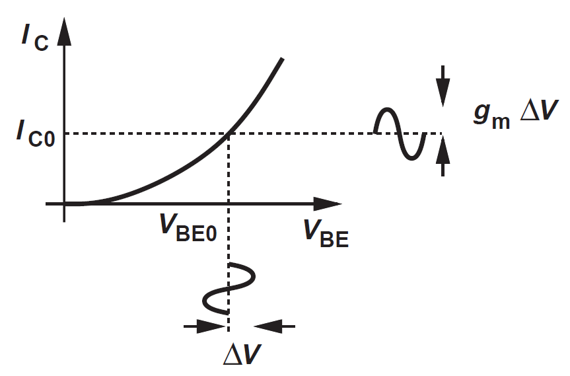
\includegraphics[width=\textwidth]{figuras/curva_transconductancia.png}
\end{figure}

\end{column}
\begin{column}{0.5\textwidth}

\begin{align*}
g_m &= \left. \dfrac{dI_C}{dV_{BE}} \right|_Q \\
g_m &= \dfrac{d}{dV_{BE}} \left\{ I_S \cdot e^{V_{BE/V_t}} \right\} \\
g_m &= I_S \cdot e^{V_{BE}/V_t} \cdot \dfrac{1}{V_t} \\
g_m &= \dfrac{I_C}{V_t} \\
\end{align*}

\end{column}
\end{columns}
    
\end{frame}


\begin{frame}{Transconductancia por expansión de serie de Taylor}

\begin{columns}
\begin{column}{0.5\textwidth}
\[ e^x = \sum_{n=0}^{\infty} \dfrac{x^n}{n!} \]
\[ e^x = 1 + \dfrac{x}{1!} + \dfrac{x^2}{2!} + \dfrac{x^3}{3!} + ... \]
\[ I_C(t) = I_S e^{(V_{BE} + v_{be}(t))/V_t} \]
\[ I_C(t) = I_S \cdot e^{V_{BE}/V_t} \cdot e^{v_{be}(t)/V_t} \]
\[ I_C(t) = I_C \cdot e^{v_{be}(t)/V_t} \]
Tomando $x = v_{be}(t)/V_t$:
\[ I_C(t) = I_C \cdot e^{x} \]

\end{column}
\begin{column}{0.5\textwidth}
La expansión de Taylor:
\[ I_C(t) = I_C \left[ 1 + \dfrac{x}{1!} + \dfrac{x^2}{2!} + ... \right] \]
Tomando sólo los términos lineales:
\[ I_C(t) = I_C \left[ 1 + \dfrac{x}{1!} \right] \]
\[ I_C(t) = I_C \left[ 1 + \dfrac{v_{be}(t)}{V_t} \right] \]
\[ I_C(t) = I_C + \dfrac{I_C}{V_t} \cdot v_{be}(t) \]
\[ I_C(t) = I_C + g_m \cdot v_{be}(t) \]
\end{column}
\end{columns}
    
\end{frame}


\section{Modelo pi}
\begin{frame}{Modelo de pequeña señal}

\begin{columns}
\begin{column}{0.5\textwidth}

En pequeña señal (corriente alterna), la corriente de colector es función de la transconductancia. 

\vspace{5mm}El modelo $\pi$ del transistor BJT tipo NPN:

\begin{figure}
    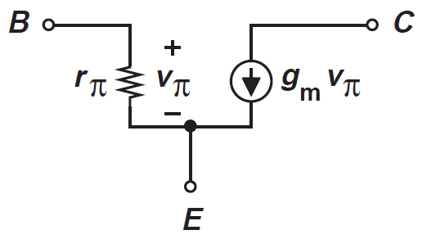
\includegraphics[width=\textwidth]{figuras/modelo_pequena_senal.png}
\end{figure}

\end{column}
\begin{column}{0.5\textwidth}

    Se definen los parámetros de pequeña señal:

    \[ g_m = \dfrac{I_C}{V_t} \]
    \[ r_\pi = \dfrac{\beta}{g_m} \]

\begin{itemize}
    \item Las variables en mayúscula ($I_C$, $V_{BE}$) describen parámetros de corriente directa.
    \item Las variables en minúscula ($i_c$, $v_{be}$) describen parámetros de corriente alterna.
\end{itemize}



\end{column}
\end{columns}
    
\end{frame}


\begin{frame}{Análisis de circuitos por superposición de fuentes}

Si un circuito tiene fuentes de CD y CA, se debe resolver por superposición de fuentes.

\begin{itemize}
    \item Primero se analiza en \textbf{Gran Señal (CD)}, con las fuentes de CA apagadas.
    \item Luego se analiza en \textbf{Pequeña Señal (CA)}, con las fuentes de CD apagadas.
\end{itemize}

\begin{figure}
    \centering
    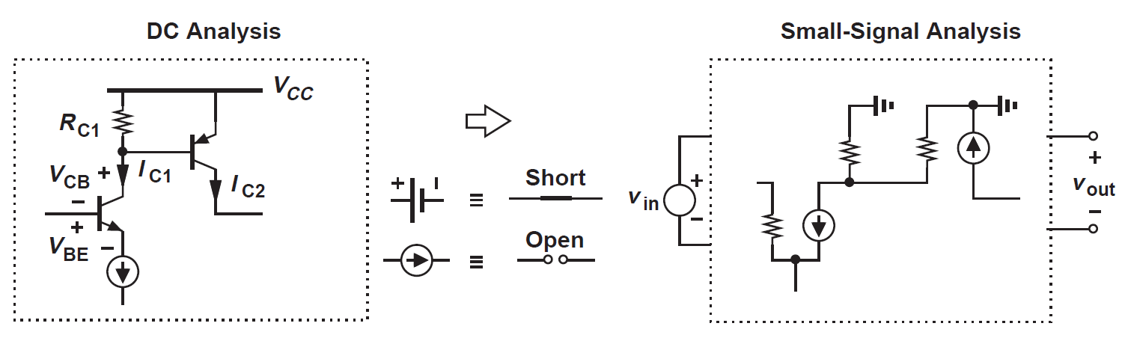
\includegraphics[width=\textwidth]{figuras/gran_senal_pequena_senal.png}
\end{figure}

\end{frame}


\section{Ejemplo 1}
\begin{frame}{Ejemplo 1: Análisis de gran señal y pequeña señal}

Determine la corriente $I_C$ en miliamperios, y la corriente $i_c(t)$ en notación fasorial.

\begin{columns}
\begin{column}{0.5\textwidth}

\begin{figure}[H]
    \centering
    \scalebox{0.8}{
    \begin{circuitikz}
        \draw (0,0) node[npn](Q1){};
        \draw (-2,0) -- (Q1.base);
        \draw (-2,0) to[V,l=$V_{CD}$] (-2,-1.5);
        \draw (-2,-1.5) to[sV,l=$v_{ca}(t)$] (-2,-3);
        \draw (-2,-3) node[ground]{};
        \draw (0,-3) node[ground]{};
        \draw (0,-3) -- (Q1.emitter);
        \draw (0,2.5) to[R,l=$R_C$] (Q1.collector);
        \draw (0,2.5) node[vcc]{};
        \draw (0,3) node[above]{$V_{CC}$};
    \end{circuitikz}}
\end{figure}

\end{column}
\begin{column}{0.5\textwidth}

\[ V_{CD} = 0.68\ V \]
\[ v_{ca}(t) = 10\ mV \sin \omega t \]
\[ I_S = 10^{-14}\ A \]
\[ \beta = 100 \]
\[ V_t = 26\ mV \]
\[ V_{CC} = 3\ V \]
\[ R_C = 100\ \Omega \]

\end{column}
\end{columns}
    
\end{frame}


\begin{frame}{Solución 1: Análisis de gran señal}

\begin{columns}
\begin{column}{0.5\textwidth}

\begin{figure}[H]
    \centering
    \scalebox{0.8}{
    \begin{circuitikz}
        \draw (0,0) node[npn](Q1){};
        \draw (-2,0) -- (Q1.base);
        \draw (-2,0) to[V,l=$V_{CD}$] (-2,-1.5);
        \draw (-2,-2) to[short,l=$v_{ca}(t)$,*-*] (-2,-2.5);
        \draw (-2,-1.5) to[short] (-2,-2);
        \draw (-2,-2.5) to[short] (-2,-3);
        \draw (-2,-3) node[ground]{};
        \draw (0,-3) node[ground]{};
        \draw (0,-3) -- (Q1.emitter);
        \draw (0,2.5) to[R,l=$R_C$] (Q1.collector);
        \draw (0,2.5) node[vcc]{};
        \draw (0,3) node[above]{$V_{CC}$};
    \end{circuitikz}}
\end{figure}

\end{column}
\begin{column}{0.5\textwidth}
El punto de operación en CD:

\[ I_C = I_S \cdot e^{V_{BE}/V_t} \]
\[ I_C = 10^{-14}\ A \cdot e^{0.68\ V/26\ mV} \]
\[ I_C = 2.28\ mA \]

\vspace{5mm}Los parámetros de pequeña señal:

\[ g_m = \dfrac{I_C}{V_t} = \dfrac{2.28\ mA}{26\ mV} = 87\ mS \]
\[ r_\pi = \dfrac{\beta}{g_m} = \dfrac{100}{87\ mS} = 1.15\ k\Omega \]

\end{column}
\end{columns}
    
\end{frame}


\begin{frame}{Solución 1: Análisis de pequeña señal}

\begin{columns}
\begin{column}{0.5\textwidth}

\begin{figure}[H]
    \centering
    \scalebox{0.8}{
    \begin{circuitikz}
        \draw (0,0) node[npn](Q1){};
        \draw (-2,0) -- (Q1.base);
        \draw (-2,-0.5) to[short,l=$V_{CD}$,*-*] (-2,-1);
        \draw (-2,0) to[short] (-2,-0.5);
        \draw (-2,-1) to[short] (-2,-1.5);
        \draw (-2,-1.5) to[sV,l=$v_{ca}(t)$] (-2,-3);
        \draw (-2,-3) node[ground]{};
        \draw (0,-3) node[ground]{};
        \draw (0,-3) -- (Q1.emitter);
        \draw (0,2.5) to[R,l=$R_C$] (Q1.collector);
        \draw (0,2.5) node[ground,rotate=180]{};
    \end{circuitikz}}
\end{figure}

\end{column}
\begin{column}{0.5\textwidth}
En corriente alterna:

\begin{figure}[H]
    \centering
    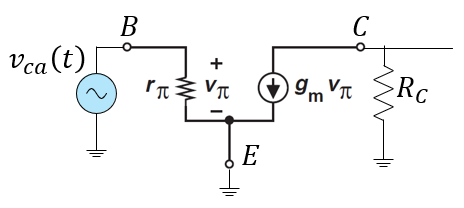
\includegraphics[width=0.8\textwidth]{figuras/ejemplo_1_modelo_peq_senal.png}
\end{figure}
%
\[ v_\pi = v_{ca}(t) = 10\ mV \angle 0^{\circ} \]

\[ i_c(t) = g_m v_\pi \]
\[ i_c(t) = 87\ mS \cdot 10\ mV \angle 0^{\circ} \]
\[ i_c(t) = 870\ mA \angle 0^{\circ} \]

\end{column}
\end{columns}
    
\end{frame}


\section{Amplificadores}
\begin{frame}{Amplificadores BJT}

\begin{itemize}
    \item Un amplificador se representa por un triángulo.
    \item Dos puertos: entrada y salida.
\end{itemize}

\begin{columns}
\begin{column}{0.5\textwidth}

\begin{figure}[H]
    \centering
    \begin{circuitikz}
        \draw (0,0) node[plain mono amp](A1){$A_V$};
        \draw (-2,0) node[left]{$v_{in}$};
        \draw (-2,0) -- (A1.in);
        \draw (2,0) -- (A1.out);
        \draw (2,0) node[right]{$v_{out}$};
    \end{circuitikz}
\end{figure}

Se define la ganancia de tensión:
\[ A_V = \dfrac{v_{out}}{v_{in}} \]

\end{column}
\begin{column}{0.5\textwidth}
Los amplificadores se construyen utilizando circuitos que convierten una tensión de entrada a corriente de salida, y luego pasan la corriente de salida a tensión de salida utilizando RL.

\vspace{3mm}Ejemplo:
\begin{figure}[H]
    \centering
    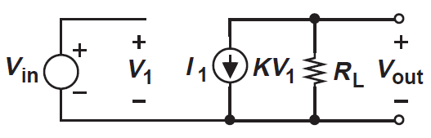
\includegraphics[width=\textwidth]{figuras/ejemplo_amplificador.png}
\end{figure}

\end{column}
\end{columns}
    
\end{frame}


\begin{frame}{Efecto de impedancias no ideales}

Si se conecta una fuente con $R_S$ y una carga $R_L$: la ganancia total se pierde.
%
\begin{columns}
\begin{column}{0.55\textwidth}
%
\begin{figure}[H]
    \centering
    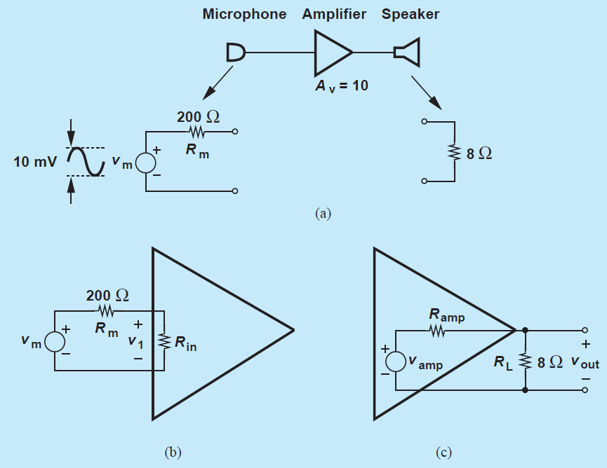
\includegraphics[width=\textwidth]{figuras/amplificador_impedancias.png}
\end{figure}

\end{column}
\begin{column}{0.45\textwidth}

\[ v_1 = \dfrac{v_m \times R_{in}}{R_S + R_{in}} \]
\[ v_{amp} = v_1 \times A_V \]
\[ v_{out} = \dfrac{v_{amp} \times R_L}{R_{out} + R_L} \]

\begin{itemize}
    \item La impedancia de un micrófono \textbf{Sennheiser e 935} es de $350\ \Omega$.
    \item La impedancia de un par de audífonos es de $32\ \Omega$ por canal.
\end{itemize}
\end{column}
\end{columns}
    
\end{frame}


\begin{frame}{Cálculo de impedancias de entrada y salida}

Para determinar la impedancia desde cualquier terminal, se conecta una fuente de prueba $v_x$ y se determina la corriente $i_x$.

\begin{figure}
    \centering
    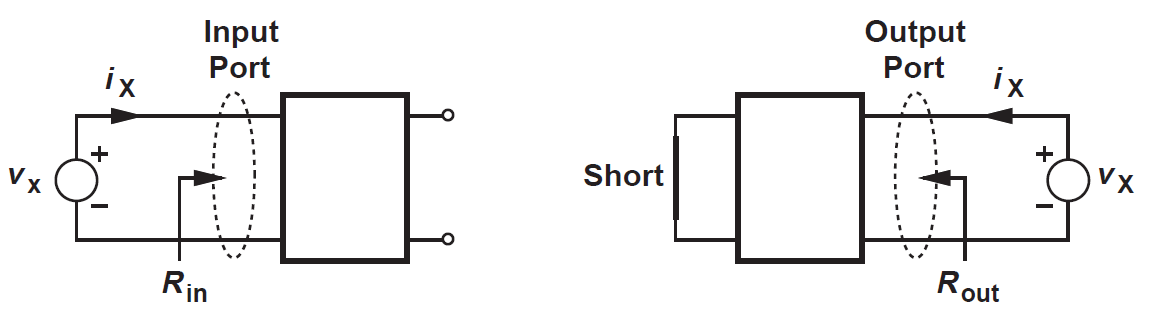
\includegraphics[width=\textwidth]{figuras/amplificador_impedancias_2.png}
\end{figure}

\begin{columns}
\begin{column}{0.5\textwidth}
\centering
La impedancia de entrada se mide con la salida en circuito abierto.
\end{column}
\begin{column}{0.5\textwidth}
\centering
La impedancia de salida se mide con la entrada en corto circuito.
\end{column}
\end{columns}
    
\end{frame}


\section{Emisor común}
\begin{frame}{Emisor Común: Ganancia}

\vspace{-5mm}\begin{columns}
\begin{column}{0.5\textwidth}

\begin{figure}[H]
    \centering
    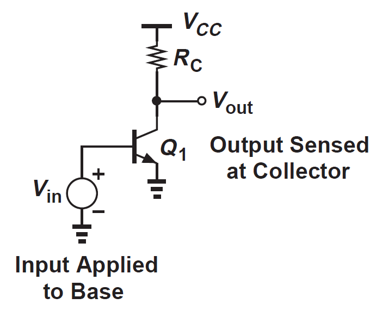
\includegraphics[width=\textwidth]{figuras/emisor_comun_circuito.png}
\end{figure}

\end{column}
\begin{column}{0.5\textwidth}

\begin{figure}[H]
    \centering
    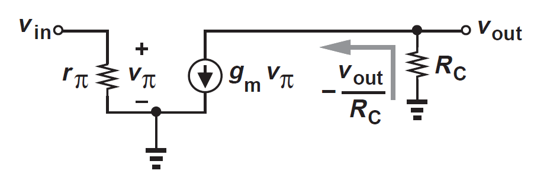
\includegraphics[width=\textwidth]{figuras/emisor_comun_ganancia.png}
\end{figure}

\end{column}
\end{columns}
    
\end{frame}


\begin{frame}{Emisor Común: Impedancias}

\begin{columns}
\begin{column}{0.5\textwidth}
\end{column}
\begin{column}{0.5\textwidth}
\end{column}
\end{columns}
    
\end{frame}


\section{Base común}
\begin{frame}{Base Común: Ganancia}

\vspace{-5mm}\begin{columns}
\begin{column}{0.5\textwidth}

\begin{figure}[H]
    \centering
    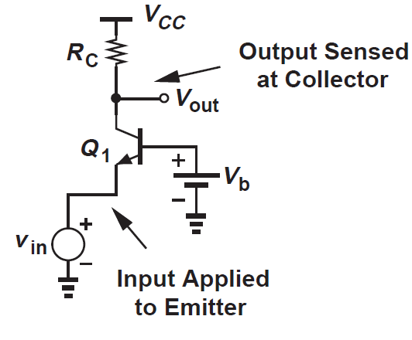
\includegraphics[width=\textwidth]{figuras/base_comun_circuito.png}
\end{figure}

\end{column}
\begin{column}{0.5\textwidth}

\begin{figure}[H]
    \centering
    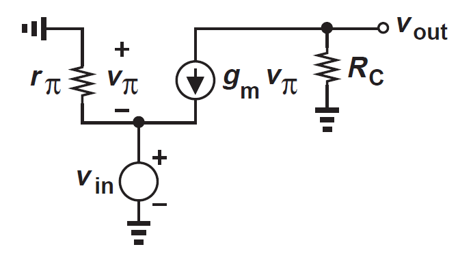
\includegraphics[width=0.8\textwidth]{figuras/base_comun_ganancia.png}
\end{figure}

\end{column}
\end{columns}
    
\end{frame}


\begin{frame}{Base Común: Impedancias}

\begin{columns}
\begin{column}{0.5\textwidth}
\end{column}
\begin{column}{0.5\textwidth}
\end{column}
\end{columns}
    
\end{frame}


\section{Colector común}
\begin{frame}{Colector Común: Ganancia}

\vspace{-5mm}\begin{columns}
\begin{column}{0.5\textwidth}

\begin{figure}[H]
    \centering
    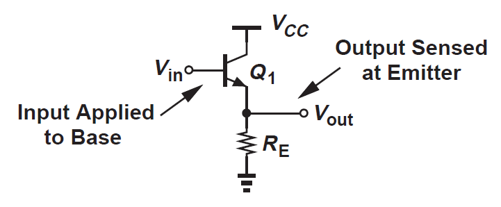
\includegraphics[width=\textwidth]{figuras/colector_comun_circuito.png}
\end{figure}

\end{column}
\begin{column}{0.5\textwidth}

\begin{figure}[H]
    \centering
    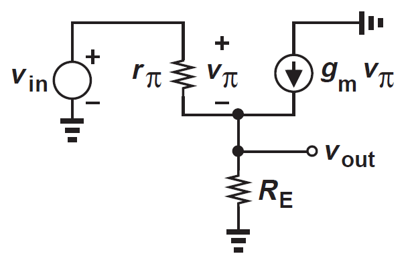
\includegraphics[width=0.8\textwidth]{figuras/colector_comun_ganancia.png}
\end{figure}

\end{column}
\end{columns}
    
\end{frame}


\begin{frame}{Colector Común: Impedancias}

\begin{columns}
\begin{column}{0.5\textwidth}
\end{column}
\begin{column}{0.5\textwidth}
\end{column}
\end{columns}
    
\end{frame}


\begin{frame}{Lecturas recomendadas}

\begin{itemize}
    \item Razavi, B. (2013). Fundamentals of Microelectronics, 2nd edition. Chapter 4: Physics of Bipolar Transistors, pp. 139-144, Wiley, Los Angeles, California.
    \item Razavi, B. (2013). Fundamentals of Microelectronics, 2nd edition. Chapter 5: Bipolar Amplifiers, pp. 171-177, Wiley, Los Angeles, California.
\end{itemize}
    
\end{frame}



\end{document}
